%%%%
% Consiglio la visione dei seguenti tutorial:
% - https://www.youtube.com/watch?v=ihxSUsJB_14
% - https://www.youtube.com/watch?v=XTFWaV55uDo
%%%%
\documentclass[12pt,a4paper,openright,twoside]{book}
\usepackage[utf8]{inputenc}

\newcommand{\thesislang}{italian} % decommentare in caso di tesi in italiano
% \newcommand{\thesislang}{english} % commentare in caso di tesi in italiano
\usepackage{thesis-style}

\begin{document}
	
\frontmatter

% ! TeX root = thesis-main.tex
\title{Title}
\author{Candidate Name Here}
\date{\today}

\newgeometry{margin=0.8in}
\begin{titlepage}
	\begin{center}
		% \vspace*{0.2cm}
		
		\large
		\textbf{ALMA MATER STUDIORUM -- UNIVERSITÀ DI BOLOGNA \\ CAMPUS DI CESENA}
		\\
		\noindent\hrulefill
		\vspace{0.4cm}
		
		\Large
		Scuola di Ingegneria e Architettura \\
		Corso di Laurea (Magistrale) in Ingegneria e Scienze Informatiche
		
		\Huge
		\vspace{4cm}
		\textbf{
			Title Thesis Here
			\\
			Long Titles Should Be Split
			\\
			On Multiple Lines
		}
		
		\large
		\vspace{1cm}
		Tesi di laurea in 
		\\
		\textsc{(Materia di Riferimento)}
		
		\vspace{5.5cm}
		\begin{minipage}[t]{0.64\textwidth}
			\begin{flushleft}
				\textit{Relatore} 
				\\ 
				(\textbf{Prof.} $\mid$ \textbf{Dott.}) \textbf{Nome Cognome}
				\\
				\vspace{0.4cm}
				\textit{Correlatore} 
				\\
				(\textbf{Ing.})? \textbf{Dott.} \textbf{Nome Cognome}
			\end{flushleft}
		\end{minipage}
		\begin{minipage}[t]{0.34\textwidth}
			\begin{flushright}
				\textit{Candidato} 
				\\ 
				\textbf{Nome Cognome}
			\end{flushright}
		\end{minipage}\\
		
		\vfill
		\noindent\hrulefill
		\vspace{0.3cm}
		\Large
		
		(N-Esima) Sessione di Laurea
		\\
		Anno Accademico 20XX-20YY
	\end{center}
\end{titlepage}
\restoregeometry


% \begin{abstract}	
% Max 2000 characters, strict.
% \end{abstract}

% \begin{dedication} % this is optional
% Optional. Max a few lines.
% \end{dedication}

% \begin{acknowledgements} % this is optional
% Optional. Max 1 page.
% \end{acknowledgements}

%----------------------------------------------------------------------------------------
\tableofcontents   
%\listoffigures     % (optional) comment if empty
%\lstlistoflistings % (optional) comment if empty
%----------------------------------------------------------------------------------------

\mainmatter

%----------------------------------------------------------------------------------------
\chapter{\introductionname}
\label{chap:introduction}

\subsection{ICOS}

Il livello dei gas serra nell'atmosfera cresce costantemente, riscaldando il nostro pianeta. Osservare 
i livelli di emissioni di questi gas è essenziale per contrastare il cambiamento climatico e mitigarne le 
conseguenze. \\

Il sistema ICOS (Integrated Carbon Observation System) è un sistema europeo creato nel 2007 come parte della ricerca 
ambientale europea, con l'obiettivo di sviluppare una rete di osservazione del carbonio in Europa
in grado di monitorare le emissioni e gli assorbimenti di CO2, nonché di altri gas serra,
in ambienti terrestri e marini. \\

ICOS si basa su una vasta rete di stazioni di misura che coprono tutta l'Europa e che forniscono 
dati di alta qualità sul bilancio del carbonio. Queste stazioni di misura sono distribuite in 
tutta Europa in modo da rappresentare una vasta gamma di ambienti, come foreste, prati, paludi,
zone umide, fiumi e oceani. Le stazioni utilizzano tecnologie avanzate per misurare il flusso
di gas serra in queste diverse ambientazioni, come ad esempio la tecnologia di campionamento 
automatico per l'acqua e l'aria, la misurazione del radon e la tecnologia satellitare.\\

ICOS raccoglie questi dati ambientali per valutare l'impatto del cambiamento climatico
sul ciclo del carbonio e per sviluppare strategie per mitigare l'impatto delle attività
umane sul clima. La raccolta e l'analisi dei dati di ICOS sono supportati da tecnologie 
avanzate del web semantico, che consentono la gestione, l'analisi e la condivisione dei dati 
ambientali in modo efficace ed efficiente. \\

ICOS è stato sviluppato in collaborazione con altri sistemi di osservazione globale del carbonio,
come il Global Carbon Project e il Copernicus Climate Change Service.
Il sistema ICOS è stato riconosciuto come una risorsa essenziale per la comprensione
del bilancio del carbonio in Europa e nel mondo, e il suo contributo è stato riconosciuto
dalla comunità scientifica e dalle organizzazioni internazionali, come il Panel Intergovernativo
sui Cambiamenti Climatici (IPCC) e l'Organizzazione per la Cooperazione e lo Sviluppo Economico (OCSE). \\

\subsection{Structure}

Il progetto ICOS è suddiviso in tre domini: \textbf{Atmosfera} - \textbf{Ecosistema} - \textbf{Oceano}. \\

L'unità fondamentale di ICOS sono le \textbf{ICOS Station Networks} che sono coordinate e gestite dall'
\textbf{ICOS National Networks}. \\

Le \textbf{MSA} (\textit{Monitoring Station Assembly}) sono assemble che studiano e discutono come migliorare
l'osservazione degli ambienti nelle stazioni, cercando di portare novità sia dal punto di vista tecnico che scientifico.
È presente un MSA per ognuno dei tre domini. \\

Le \textbf{Central Facilities} sono entità che coordinano il supporto alle stazione. Ogni dominio ha la sua Central Facility. \\

\begin{figure}[H]
    \caption{ICOS structure}
    \centering
    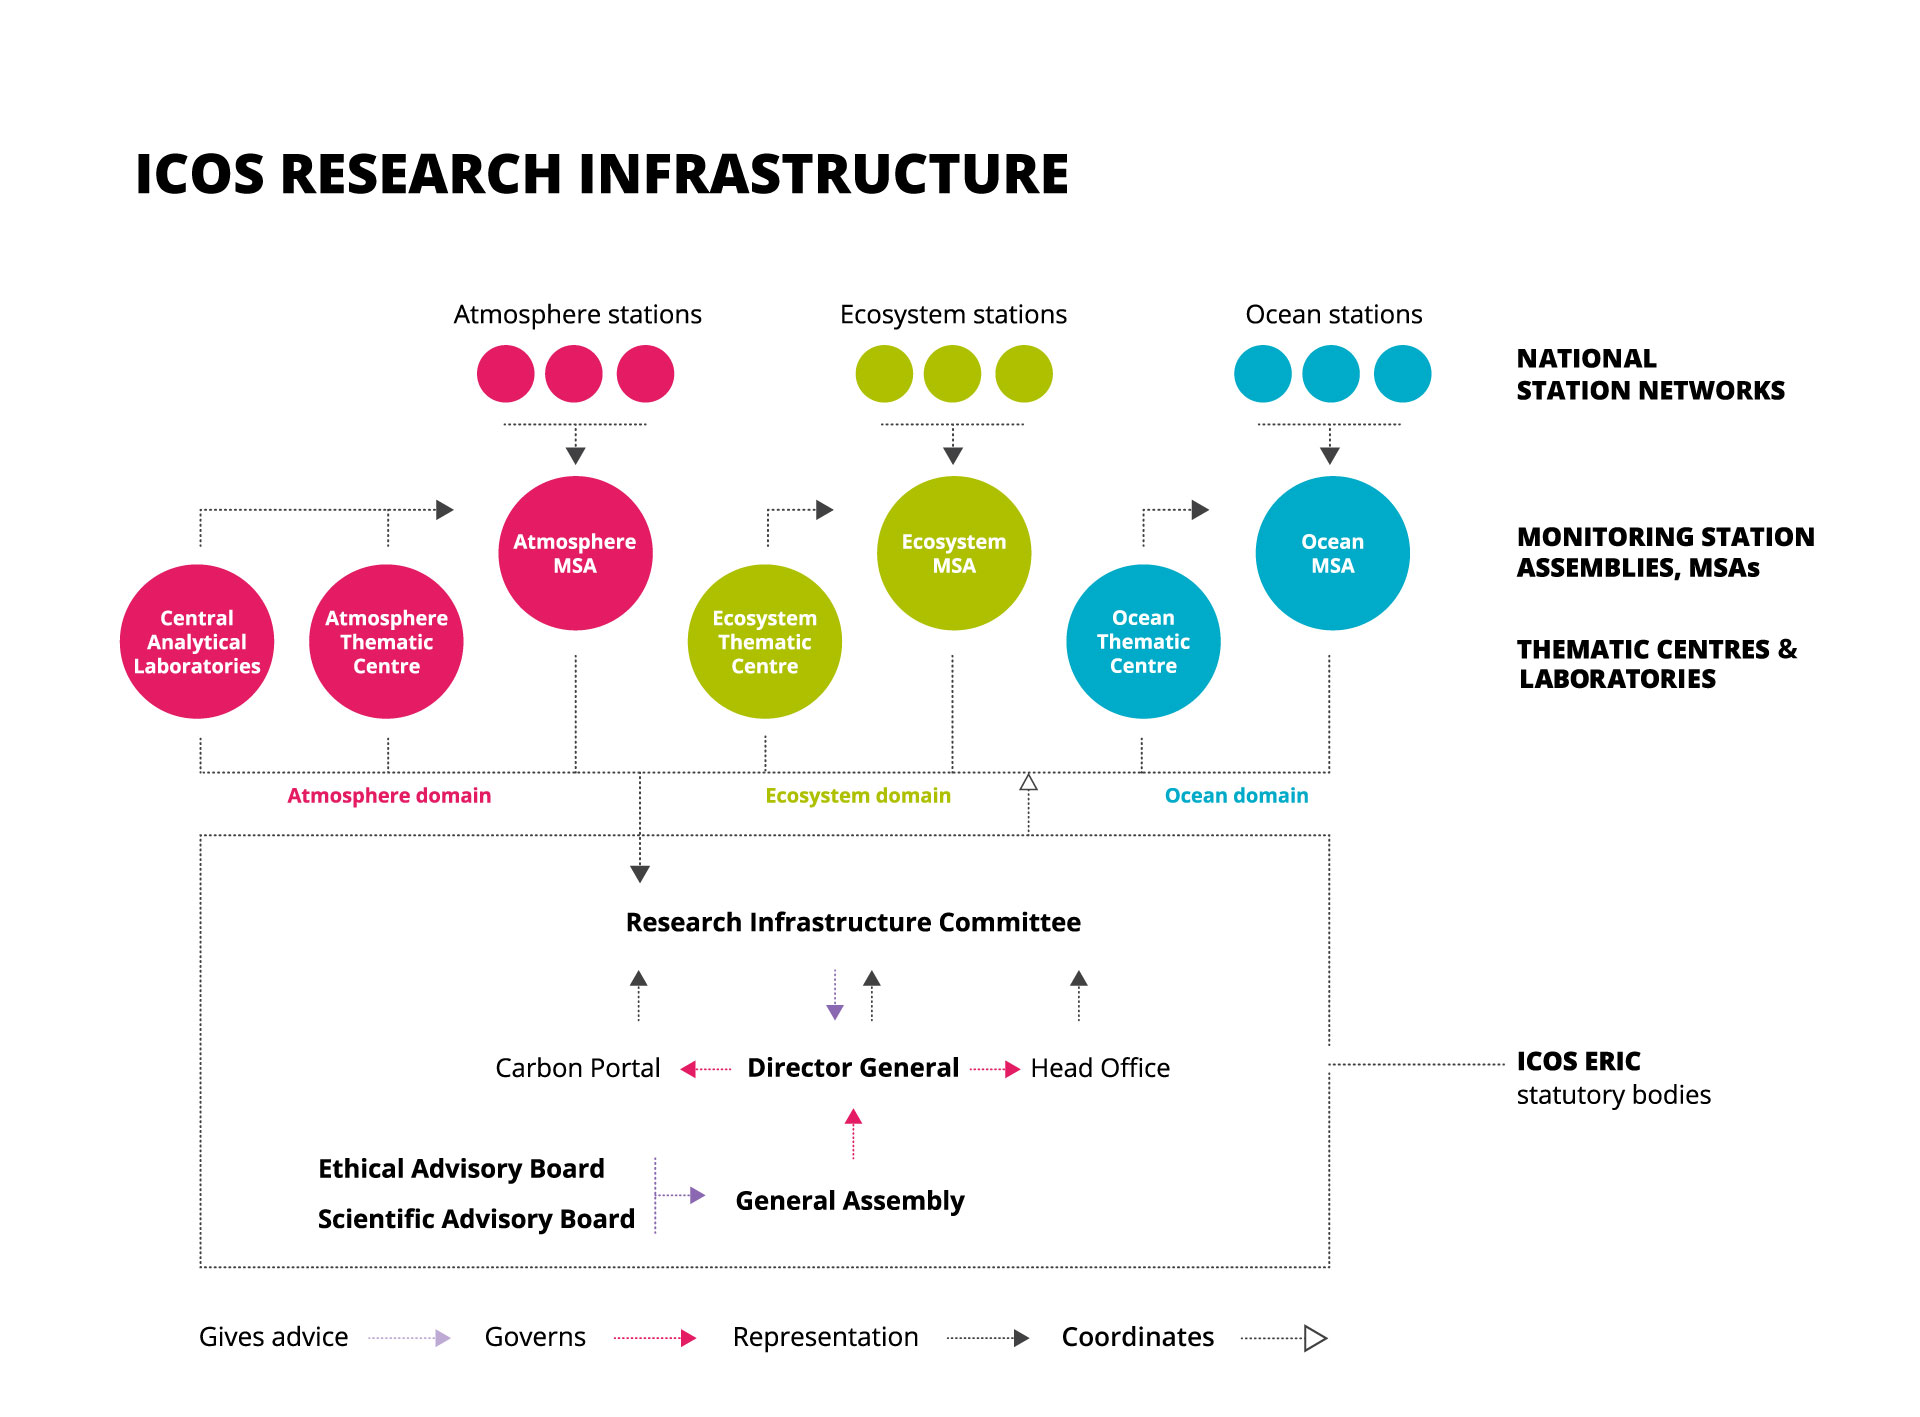
\includegraphics[width=\textwidth]{figures/icos-structure.png}
\end{figure}
%----------------------------------------------------------------------------------------
\chapter{Dati utilizzati}
\label{chap:dati}

Il progetto ICOS fornisce dati standardizzati e di altas qualità sui gas a effetto serra.
Tutti i dati sono accessibili attraverso la licenza \textit{Creative Commons Attribution 4.0 International license}.
La licenza Creative Commons 4.0 permette di condividere e utilizzare opere originali in modo più flessibile rispetto
al diritto d'autore tradizionale, ma con alcune limitazioni e requisiti per garantire il rispetto dei diritti dell'autore originale.

\section{FAIR principles}
\label{section:fair}
I dati prodotti da ICOS seguono i cosidetti principi \textbf{FAIR}.
I principi FAIR mirano a fornire all'utente strumenti sufficienti per 
comprendere il significato dei dati prima e dopo averli scaricati. 
I principi FAIR definiscono quindi dei requisiti fondamentali per
la gestione dei dati scientifici, al fine di renderli "FAIR",
ovvero Findable (Rintracciabili), Accessible (Accessibili), Interoperable (Interoperabili) e 
Reusable (Riutilizzabili). A tale scopo, ICOS utilizza la tecnologia dei \textit{Linked-Open Data} \ref{section:linkeddata},
tecnologia moderna e avanzata nel campo della gestione dati. 

I quattro principi FAIR sono i seguenti:

\begin{itemize}
    \item Findable: i dati scientifici devono essere facilmente identificabili e rintracciabili attraverso i metadati appropriati.
    Ciò implica l'utilizzo di identificatori univoci e di descrizioni dettagliate dei dati.
    \item Accessible: i dati scientifici devono essere accessibili in modo aperto e gratuito.
    Ciò implica l'utilizzo di licenze adeguate e la disponibilità di strumenti e tecnologie per accedere ai dati.
    \item Interoperable: i dati scientifici devono essere interoperabili, ovvero strutturati in modo standard
    e condivisibili con altre fonti di dati. Ciò implica l'utilizzo di formati standard, di ontologie e di protocolli
    di comunicazione comuni.
    \item Reusable: i dati scientifici devono essere riutilizzabili
    in modo flessibile e senza restrizioni, anche per scopi diversi da quelli
    per cui sono stati creati. Ciò implica la pubblicazione di dati e metadati completi,
    la documentazione dei processi di acquisizione e la creazione di strutture di dati flessibili.
\end{itemize}


\section{PIDs}
Per collegare la proprietà dei dati al dato stesso, ICOS impiega i \textbf{Persistent Identifiers (PIDs)}.
Questo identificatore univoco utilizza i \textit{DataCite Digital Object Identifiers (DOIs)} per i datasets
e le collezioni. Questi tag identificano ciascuno \textit{data object} e può essere citato, per esempio,
in una qualche pubblicazione scientifica. Il PID è creato automaticamente e immediatamente
non appena il data è caricato; inoltre il dato viene cifrato per assicurarne la validità.\\

Il PID è un indirizzo web valido (URL), che riporta ad una sua specifica landing page,
dove molteplici informazioni possono essere trovate tra cui i meta-data accessibili sia
dagli utenti che dalle macchine. L'intero processo garantisce che il dato scaricato e quello
originale sia esattamente identici con i metadati associati. Altri portali 
potrebbero usare il PID e il link associato al dato e fornire accesso trasparente al \textit{data object}
attraverso l'ICOS Carbon Portal.

\begin{figure}[h!]
    \centering
    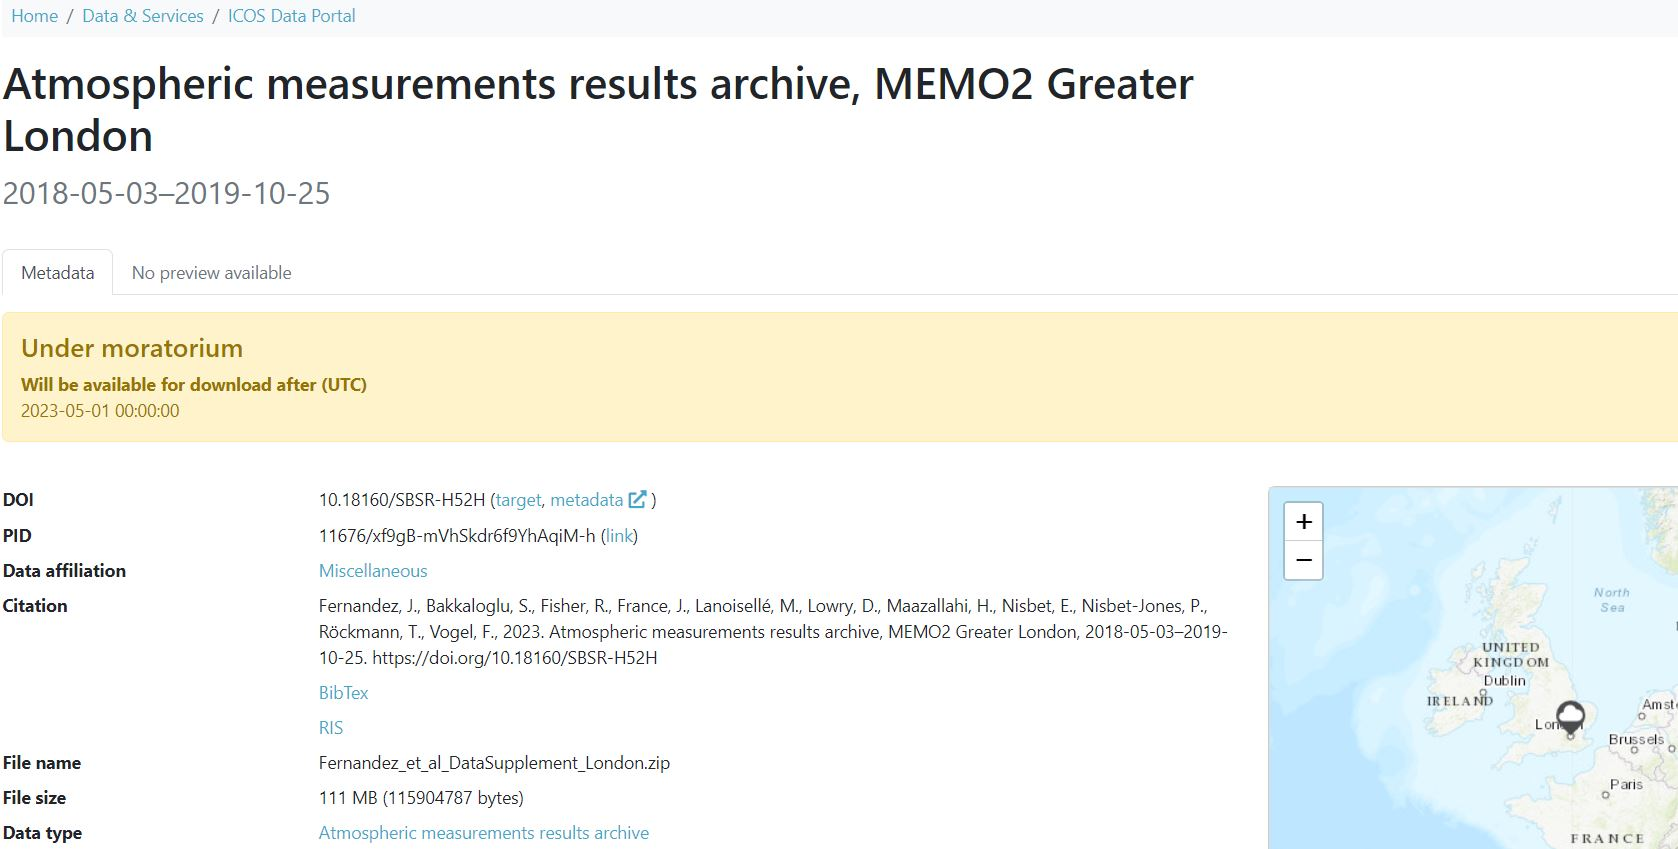
\includegraphics[width=0.7\textwidth]{figures/PIDex.JPG}
    \caption{Esempio di pagina web contentente i metadati tra cui il PID (il link della pagina) e il DOI.}
    \label{figure:PIDex}
\end{figure}

\begin{figure}[h!]
    \centering
    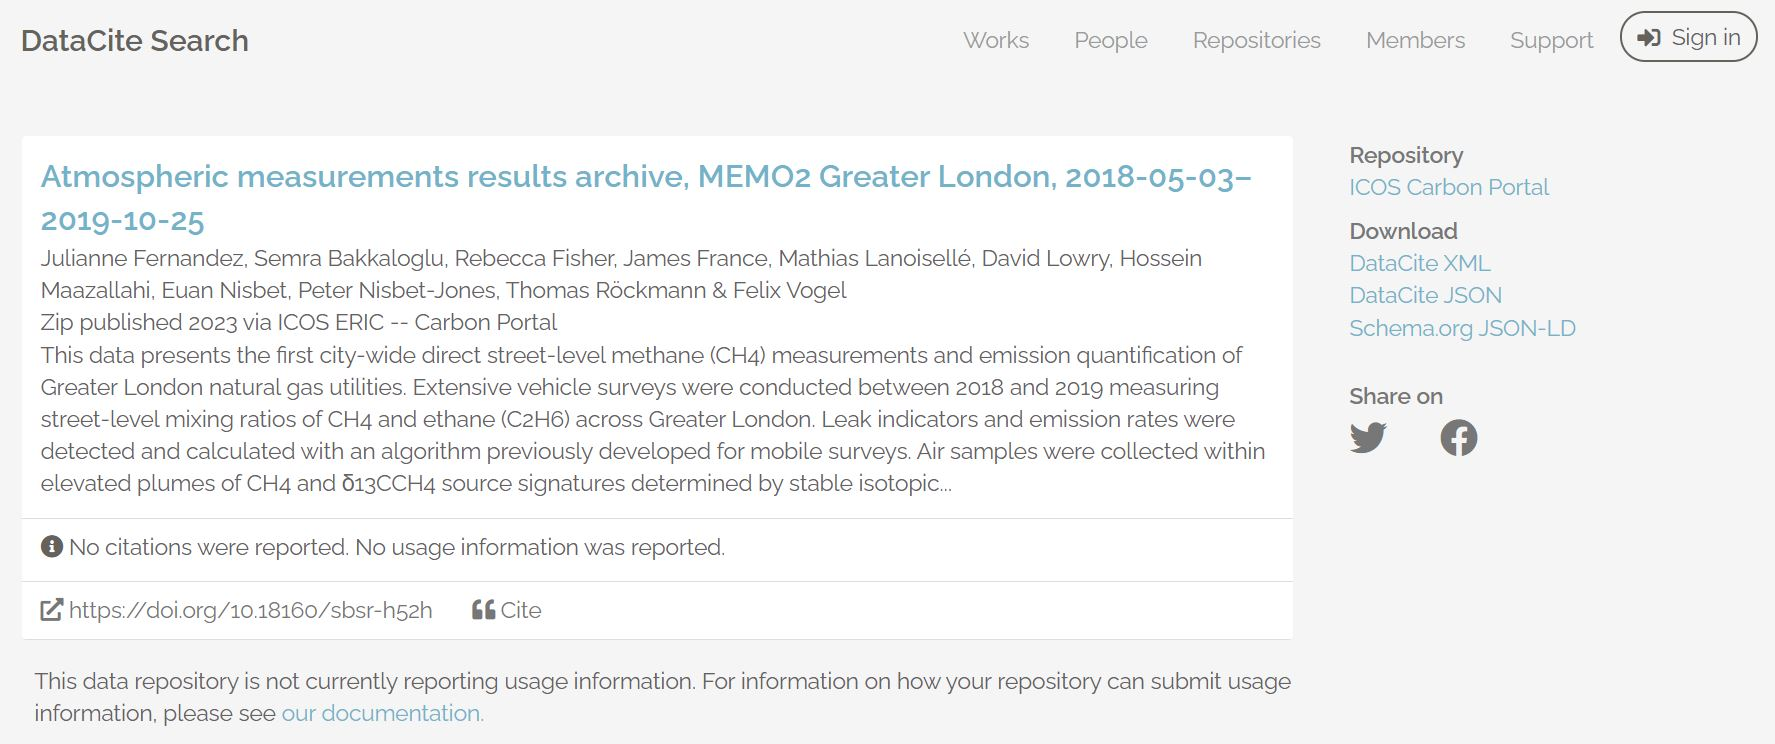
\includegraphics[width=0.7\textwidth]{figures/DOIex.JPG}
    \caption{Esempio di DOI che riporta automaticamente ad una risorsa all'intereno del dominio di DataCite.}
    \label{figure:DOIex}
\end{figure}


\section{Data-production Process}
Il processo di produzione e standardizzazione dei dati segue 11 fasi, descritte qui di seguito e nella figura \ref{figure:data-process}:
\begin{enumerate}
    \item \textit{I dati son raccolti presso le stazioni di misurazione}.
    ICOS possiede circa 150 stazioni di misurazione, suddivisi in 14 paesi,
    che formano tre reti principali di raccolta (\ref{section:thematic}, Atmosphere, Ecosystem e Ocean).
    \item \textit{I dati grezzi vengono salvati in repository sicure}.
    Essendo i dati il fulcro di questo progetto, inoltre è impossibile raccogliere nuovamente
    lo stesso dato, i dati vengono salvati entro 24 ore all'interno di
    data center sicuri.
    \item \textit{I dati vengono inoltrati al centro di interesse}. Ogni stazione manda i dati dei propri sensori al centro di interesse
    (\ref{section:thematic}, Atmosphere, Ecosystem o Ocean), che li processano ulteriormente e su cui svolgono controlli di qualità.
    \item \textit{I dati sono inoltre inviati al CAL}. Il CAL (\ref{section:CAL}, Central Analytical Laboratories)
     ha come obiettivo quello di garantire
    l'accuratezza delle misure atmosferiche nelle stazioni ICOS.
    \item \textit{Il centro di interesse elabora i dati}. Il centro di interesse che riceve i dati dovrà controllare la validità dei dati, assicurarne la qualità e
    standardizzarli. Infine, i dati vengono aggregati in gruppi di misurazioni da mezz'ora o un'ora.
    \item \textit{Dato trasferiti al Carbon Portal}. Quando i dati sono pronti vengono inviati al Carbon Portal \ref{section:carbonportal}, 
    cercando giorno dopo giorno d ridurre i tempi di delivery di questi dati.
    \item \textit{Il Carbon Portal riceve e si prende cura di tutti i datasets ICOS}. Il Carbon Portal \ref{section:carbonportal} si occuperà della gestione, dei servizi di visualizzazione e data management legati ai datasets ICOS.
    \item \textit{Gli utenti possono liberamente agire sui dati}. Chiunque voglia accedere, scaricare e visualizzare i dati potrà farlo dal Carbon Portal \ref{section:carbonportal}.
    \item \textit{Tutti gli ICOS Data Products sono in data center sicuri}. Copie di tutti i Data Product, e i relativi metadati,
    sono salvati in maniera sicura in repository dislocate geograficamente (Finalndia, Germania e centro tematico d'iteresse).
    \item \textit{Le descrizioni dei Data Products devono essere facilmente accessibili}. ICOS si impegna a diffondere tutte le informazioni relative ai Data Product.
    \item \textit{I dati ICOS devono essere inviabili agli altri centri di ricerca}. Il processo e le infrastrutture per la produzione dei dati ICOS devono fare in modo che i dati prodotti possano essere facilmente 
    trasferibili ad altri centri di ricerca che potrebbero beneficiarne.
\end{enumerate}

\begin{figure}[h!]
    \centering
    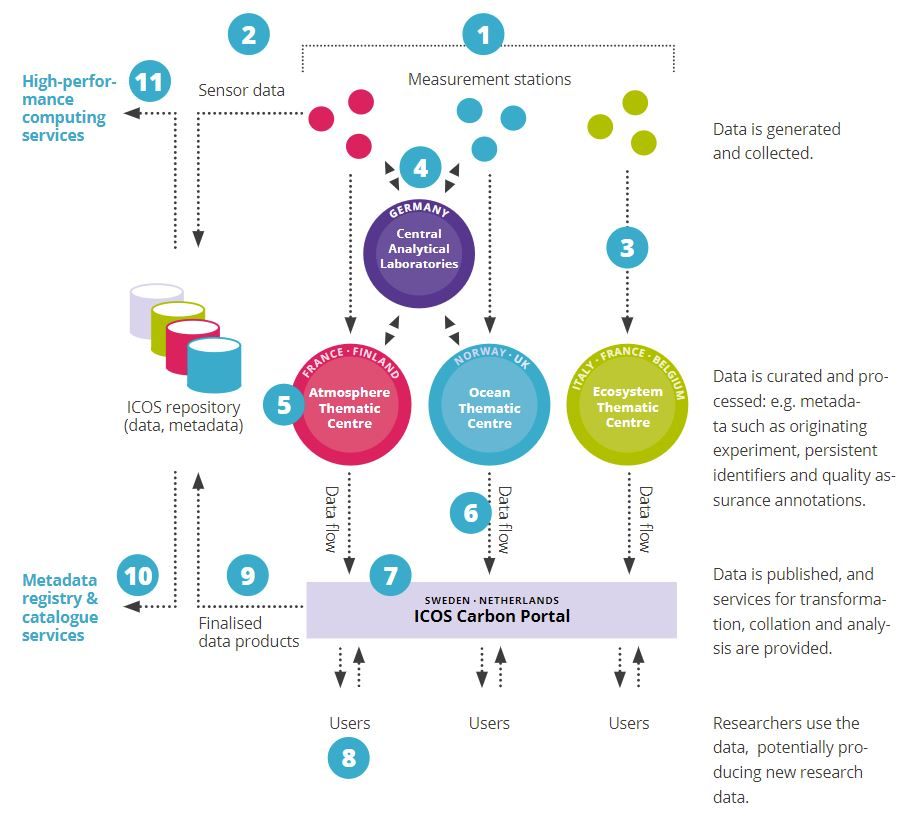
\includegraphics[width=0.8\textwidth]{figures/data-process.JPG}
    \caption{Diagramma della processo di produzione e mantenimento dei dati ICOS.}
    \label{figure:data-process}
\end{figure}


\section{Data product levels}
\label{section:data-level}
Per definire al meglio quelli che ICOS considera dati "grezzi" da dati "finiti",
questi dati sono stati raggruppati in 4 possibili livelli, a seconda della qualità.

\begin{enumerate}
    \item \textbf{Dati grezzi}. Sono i dati direttamente raccolti dai sensori delle stazioni e quindi non elaborati. Possono assumere diverse forme come immagini, testo o campioni fisici.
    \item \textbf{Livello Dati 0}. I dati di livello 0
    sono dati in unità fisiche forniti direttamente dagli
    strumenti o convertiti manualmente dal reparto
    ingegneristico (ad esempio, mV, mA) in unità fisiche
    del Centro Tematico. Potrebbero esserlo stati
    filtrati da un primo controllo qualitativo.
    \item \textbf{Livello Dati 1}. I dati di livello 1 si dividono in due sotto categorie:
        \begin{itemize}
            \item \textit{Level 1 Near Real Time data (L1\_NRT)}. Sono dati che 
            vengono generalmente distribuiti entro 24 ore dalla rilevazione,
            raggruppati in dataset di alta qualità (che quindi hanno superato
            controlli di qualità) e resi disponibili automaticamente attraverso
            il Carbon Portal.  
            \item \textit{Level 1 Internal or Intermediate Working data (L1\_IW)}.
            Questi dati sono generati dagli step intermedi per la preparazione dei dati
            NRT o di livello 2. Per questo motivo non verranno distribuiti ma rimarranno
            all'interno delle infrastrutture ICOS per controlli di qualità interni
            e torneranno utili nella produzione dei dati di livello 2.
        \end{itemize} 
    \item \textbf{Livello Dati 2}. Sono i dati finali rilasciati da ICOS dopo i più rigorosi
    controlli, accessibili sul Carbon Portal.
    \item \textbf{Livello Dati 3}. Tutti i risultati prodotti da ricercatori o enti
    terzi, quindi esterni ad ICOS, tramite dati ICOS vengono catalogati come dati di livello 3.
\end{enumerate}

\begin{figure}[h!]
    \centering
    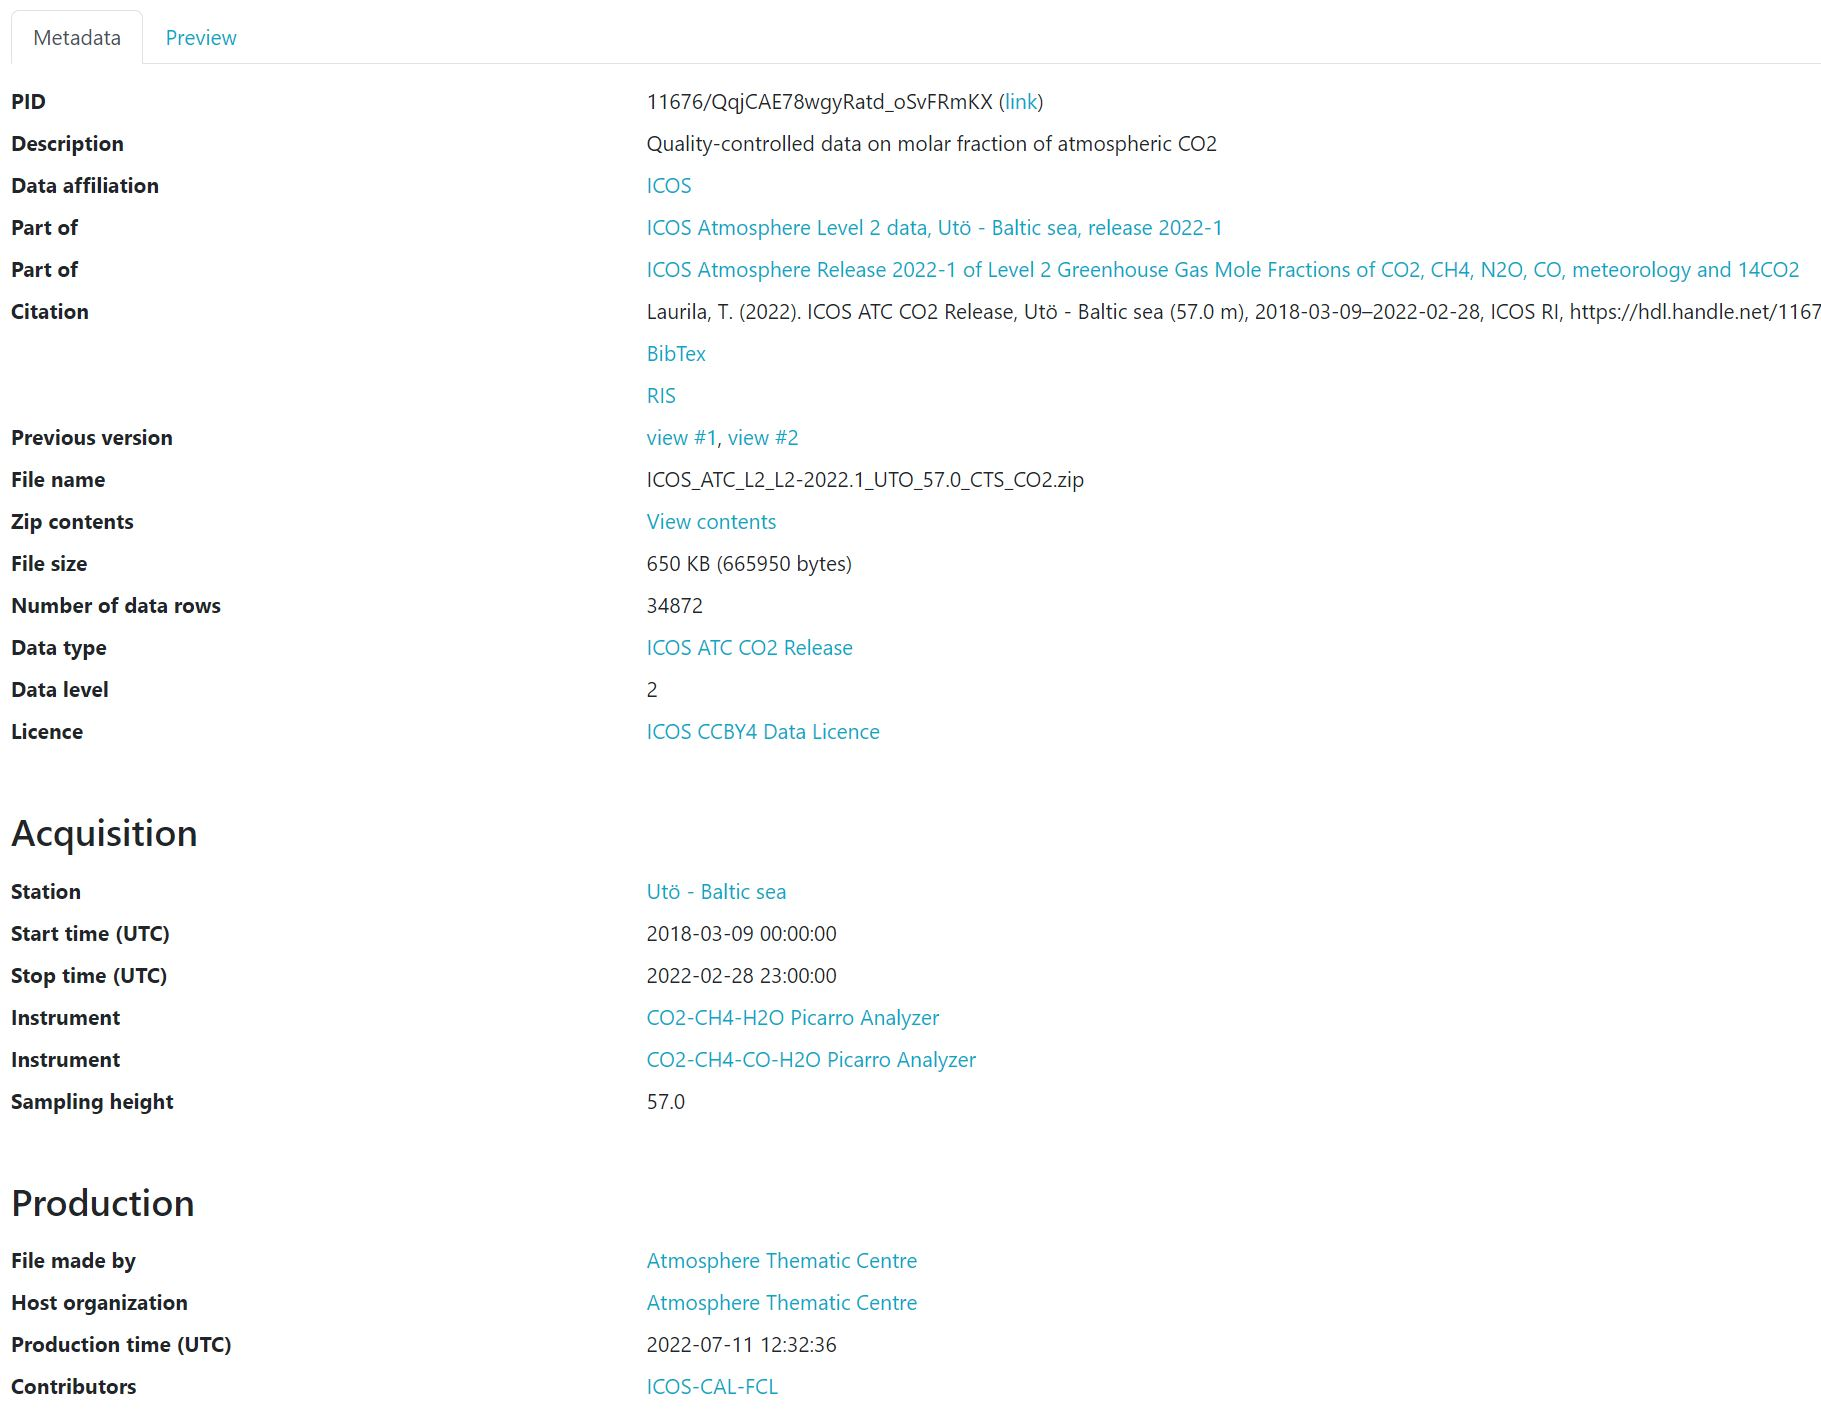
\includegraphics[height=0.36\textwidth]{figures/metaEx.JPG}
    \caption{Alcuni dei meta-data che si possono trovare nei dati ICOS: in figura si può notare tra le altre, anche il Data Level.}
    \label{figure:metadata-ex}
\end{figure}
%----------------------------------------------------------------------------------------
\chapter{Tecnologie Impiegate}
\label{chap:tecnologie}

Il progetto ICOS utilizza diverse tecnologie del web semantico per la gestione dei dati e dei metadati relativi alle misurazioni dell'anidride carbonica e di altri gas serra effettuate dalle stazioni di monitoraggio ICOS. Alcune delle principali tecnologie utilizzate sono:

\section{RDF}
\label{section:rdf}
RDF (Resource Description Framework): il progetto ICOS utilizza il
formato RDF per rappresentare i dati e i metadati relativi
alle misurazioni delle stazioni di monitoraggio.
RDF è un formato standard del web semantico utilizzato
per rappresentare le informazioni in modo strutturato.\\

In particolare ICOS utilizza sia la sintassi RDF/XML sia quella
RDF/Turtle, lasciando la possibilità all'utente di scaricare i dati
nel formato che preferiscono.

\section{OWL}
\label{section:owl}
OWL (Web Ontology Language): l'ontologia ICOS
Carbon Portal utilizza il linguaggio formale OWL
per definire i concetti e le relazioni tra i concetti.
OWL è un linguaggio standard del web semantico utilizzato
per descrivere ontologie e sviluppato dal W3C come estensione
del linguaggio RDF.\\

ICOS ha definito un vocabolario OWL per la
descrizione dei metadati dei dati raccolti
dalle stazioni di monitoraggio ICOS,
in particolare per quanto riguarda la struttura,
la qualità e le informazioni sul contesto di
acquisizione dei dati. Questa particolare ontologia non solo
viene usata da ICOS ma anche da SITES (Swedish
Infrastructure for Ecosystem Science) \cite{SITESHomepage},
l'infrastruttura nazionale svedese per la ricerca sul campo
terrestre e limnologica.

\section{SPARQL}
\label{section:sparql}
SPARQL (SPARQL Protocol and RDF Query Language): il progetto
ICOS utilizza SPARQL per interrogare e recuperare i dati e
i metadati delle stazioni di monitoraggio.
SPARQL è un linguaggio di interrogazione standard
del web semantico utilizzato per recuperare informazioni
dalle ontologie RDF.\\

Inoltre, ICOS fornisce un endpoint SPARQL pubblico,
che consente agli utenti di eseguire query SPARQL sui dati
e metadati ICOS. L'interfaccia, come si può notare in figura \ref{figure:sparqlendpoint}, permette di scrivere query personalizzate
oppure selezionarne una pre-esistente. Infine, si può liberamente
scegliere il formato del risultato ritornato dalla richiesta tra JSON,
CSV, XML e Turtle.

\begin{figure}[h!]
    \centering
    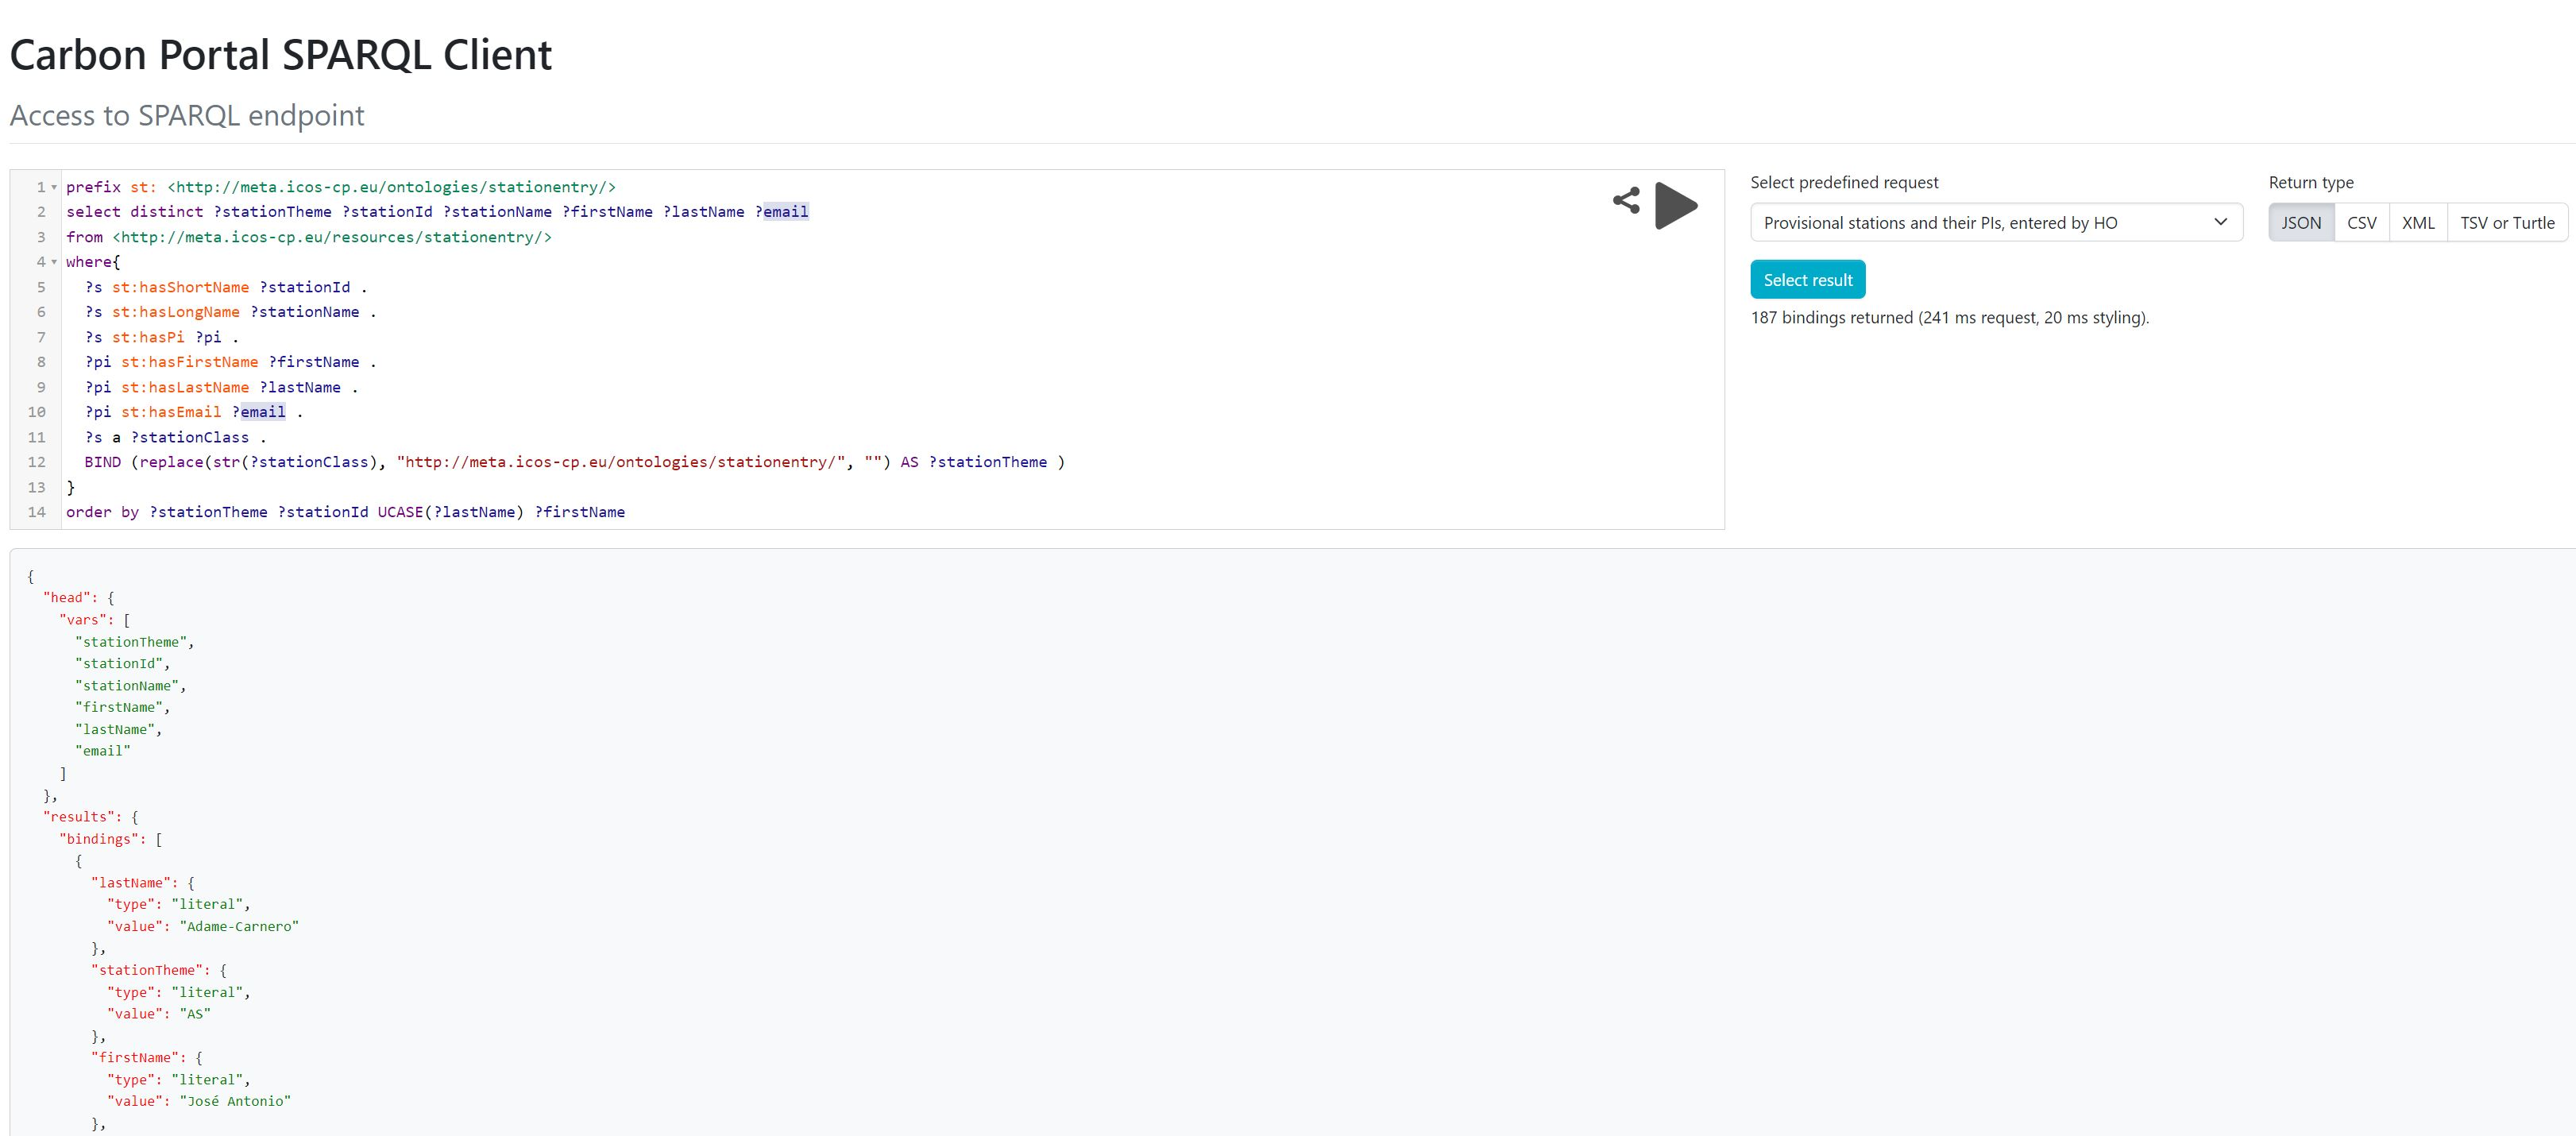
\includegraphics[width=0.8\textwidth]{figures/sparqlendpoint.JPG}
    \caption{L'endpoint SPARQL di ICOS con una query d'esempio eseguita.}
    \label{figure:sparqlendpoint}
\end{figure}

\section{Jupyter}
\label{section:jupyter}
Jupyter è un ambiente di lavoro interattivo per la creazione e condivisione di documenti che contengono codice, testo, visualizzazioni e altri elementi multimediali.
ICOS utilizza Jupyter come uno strumento fondamentale per l'analisi e la visualizzazione dei dati raccolti dalle stazioni di monitoraggio ICOS.\\

Per facilitare agli utenti l'accesso,
l'elaborazione e l'interazione con i
dati ICOS, ICOS Carbon Portal
offre diverse soluzioni tramite Jupyter \cite{JupyterICOS}.
Esistono soluzioni pre-implementate, 
che consentono la collaborazione tra
scienziati che lavorano allo
stesso progetto, condividendo dati
e codice. Inoltre, esistono soluzioni
per rispondere alle esigenze degli
scienziati che desiderano utilizzare
i dati ICOS in combinazione con
i propri dati. Infine, ICOS
Carbon Portal ha sviluppato
notebook Jupyter specifici per promuovere i dati,
i metadati e il ruolo di ICOS a
persone che potrebbero non avere
alcun collegamento diretto o
conoscenza preliminare di ICOS,
come ricercatori, responsabili politici,
educatori, studenti o persone di ogni tipo.

\section{Linked Data}
\label{section:linkeddata}
Il progetto ICOS segue il principio di Linked Data \cite{ICOSHandbook2020}, tecnologia moderna
e avanzata nel campo della gestione dati, che consente di distribuire
i dati tramite collegamenti Internet (creazione di link tra
le risorse RDF), sui quali l'utente
può semplicemente fare clic per visualizzare
e/o scaricare i dati. Ciò consente di creare
una rete di dati interconnessi
e di aumentare la loro interoperabilità. 
Inoltre, rende possibile la \textit{machine-to-machine
communication}, 
che rappresenta lo scambio di informazioni (prevalentemente
automatico,
quindi senza intervento umano) tra dispositivi di varia natura 
oppure mediante un sistema di elaborazione dati centrale.




%----------------------------------------------------------------------------------------
\chapter{\conclusionsname}
\label{chap:conclusions}
%----------------------------------------------------------------------------------------
TODO

%----------------------------------------------------------------------------------------
% BIBLIOGRAPHY
%----------------------------------------------------------------------------------------

%\nocite{*} % uncomment this to show all the reference in the .bib file
\bibliographystyle{plain}
\bibliography{bibliography}


\end{document}